\documentclass{scrartcl} % scrartcl of scrreprt
% Include all project wide packages here.
\usepackage{fullpage}
\usepackage{polyglossia}
\setmainlanguage{dutch}
\usepackage{csquotes}
\usepackage{graphicx}
\usepackage{epstopdf}
\usepackage{pdfpages}
\usepackage{caption}
\usepackage[list=true]{subcaption}
\usepackage{float}
%\usepackage{mathtools}
\usepackage{standalone}
\usepackage{import}
\usepackage{tocloft}
\usepackage{wrapfig}
\usepackage{authblk}
\usepackage{array}
\usepackage{booktabs}
\usepackage[toc,page,title,titletoc]{appendix}
\usepackage{xunicode}
\usepackage{amsmath}
\usepackage{fontspec}
\usepackage{unicode-math}
\usepackage[
    backend=bibtexu,
	texencoding=utf8,
bibencoding=utf8,
    style=ieee,
    sortlocale=nl_NL,
    language=auto
]{biblatex}
\usepackage{listings}
\newcommand{\includecode}[3][c]{\lstinputlisting[caption=#2, escapechar=, style=#1]{#3}}
\newcommand{\superscript}[1]{\ensuremath{^{\textrm{#1}}}}
\newcommand{\subscript}[1]{\ensuremath{_{\textrm{#1}}}}


\newcommand{\chapternumber}{\thechapter}
\renewcommand{\appendixname}{Bijlage}
\renewcommand{\appendixtocname}{Bijlagen}
\renewcommand{\appendixpagename}{Bijlagen}

\usepackage[hidelinks]{hyperref} %<--------ALTIJD ALS LAATSTE

\renewcommand{\familydefault}{\sfdefault}

\setmainfont[Ligatures=TeX]{Myriad Pro}
\setmathfont{Asana Math}
\setmonofont{Lucida Console}

\usepackage{titlesec, blindtext, color}
\definecolor{gray75}{gray}{0.75}
\newcommand{\hsp}{\hspace{20pt}}
\titleformat{\chapter}[hang]{\Huge\bfseries}{\chapternumber\hsp\textcolor{gray75}{|}\hsp}{0pt}{\Huge\bfseries}
\renewcommand{\familydefault}{\sfdefault}
\renewcommand{\arraystretch}{1.2}
\setlength\parindent{0pt}

%For code listings
\definecolor{black}{rgb}{0,0,0}
\definecolor{browntags}{rgb}{0.65,0.1,0.1}
\definecolor{bluestrings}{rgb}{0,0,1}
\definecolor{graycomments}{rgb}{0.4,0.4,0.4}
\definecolor{redkeywords}{rgb}{1,0,0}
\definecolor{bluekeywords}{rgb}{0.13,0.13,0.8}
\definecolor{greencomments}{rgb}{0,0.5,0}
\definecolor{redstrings}{rgb}{0.9,0,0}
\definecolor{purpleidentifiers}{rgb}{0.01,0,0.01}


\lstdefinestyle{csharp}{
language=[Sharp]C,
showspaces=false,
showtabs=false,
breaklines=true,
showstringspaces=false,
breakatwhitespace=true,
escapeinside={(*@}{@*)},
columns=fullflexible,
commentstyle=\color{greencomments},
keywordstyle=\color{bluekeywords}\bfseries,
stringstyle=\color{redstrings},
identifierstyle=\color{purpleidentifiers},
basicstyle=\ttfamily\small}

\lstdefinestyle{c}{
language=C,
showspaces=false,
showtabs=false,
breaklines=true,
showstringspaces=false,
breakatwhitespace=true,
escapeinside={(*@}{@*)},
columns=fullflexible,
commentstyle=\color{greencomments},
keywordstyle=\color{bluekeywords}\bfseries,
stringstyle=\color{bluestrings},
identifierstyle=\color{purpleidentifiers}
}

\lstdefinestyle{vhdl}{
language=VHDL,
showspaces=false,
showtabs=false,
breaklines=true,
showstringspaces=false,
breakatwhitespace=true,
escapeinside={(*@}{@*)},
columns=fullflexible,
commentstyle=\color{greencomments},
keywordstyle=\color{bluekeywords}\bfseries,
stringstyle=\color{redstrings},
identifierstyle=\color{purpleidentifiers}
}

\lstdefinestyle{xaml}{
language=XML,
showspaces=false,
showtabs=false,
breaklines=true,
showstringspaces=false,
breakatwhitespace=true,
escapeinside={(*@}{@*)},
columns=fullflexible,
commentstyle=\color{greencomments},
keywordstyle=\color{redkeywords},
stringstyle=\color{bluestrings},
tagstyle=\color{browntags},
morestring=[b]",
  morecomment=[s]{<?}{?>},
  morekeywords={xmlns,version,typex:AsyncRecords,x:Arguments,x:Boolean,x:Byte,x:Char,x:Class,x:ClassAttributes,x:ClassModifier,x:Code,x:ConnectionId,x:Decimal,x:Double,x:FactoryMethod,x:FieldModifier,x:Int16,x:Int32,x:Int64,x:Key,x:Members,x:Name,x:Object,x:Property,x:Shared,x:Single,x:String,x:Subclass,x:SynchronousMode,x:TimeSpan,x:TypeArguments,x:Uid,x:Uri,x:XData,Grid.Column,Grid.ColumnSpan,Click,ClipToBounds,Content,DropDownOpened,FontSize,Foreground,Header,Height,HorizontalAlignment,HorizontalContentAlignment,IsCancel,IsDefault,IsEnabled,IsSelected,Margin,MinHeight,MinWidth,Padding,SnapsToDevicePixels,Target,TextWrapping,Title,VerticalAlignment,VerticalContentAlignment,Width,WindowStartupLocation,Binding,Mode,OneWay,xmlns:x}
}

%defaults
\lstset{
basicstyle=\ttfamily\small,
extendedchars=false,
numbers=left,
numberstyle=\ttfamily\tiny,
stepnumber=1,
tabsize=4,
numbersep=5pt
}
\addbibresource{../../library/bibliography.bib}

\author{Xenia Wesdijk}
\title{EPO3: Eindrapport - SPI}

\begin{document}
\section{SPI}
\label{sec:spi}

%specificaties
\subsection{Specificaties}
Voor de communicatie tussen de arduïno en onze GPU hebben we een SPI decoder nodig. De ingang SS staat voor Slave Select, deze wordt normaal gebruikt voor het geval dat je meerdere slave chips hebt, aangezien dit bij ons niet het geval is zal dit signaal altijd hoog zijn. Het signaal SCLK is voor het CLK signaal voor de communicatie. Als laatste ingang is er de MOSI, dit staat voor Master Out , Slave In, dit is de daadwerkelijke dat die verzonden wordt van de arduïno naar onze GPU. Voor de uitgangen hebben we MISO, Master Input, Slave Output, dit is om de volgende instructie aan te vragen van de arduïno. Dan zijn er nog de uitgangen naar de instructie decoder, de 8 bits data bus voor om alle data te sturen als de data ready hoog is.

Ingangen: 
\begin{itemize}
	\item  MOSI
	\item SS (1 bit altijd hoog)
	\item SCLK (clk signaal)
	\item readytosend (1 bit)
\end{itemize}
Uitgangen:
\begin{itemize}
	\item MISO
	\item 8 bits data bus
	\item data ready  
\end{itemize}

%Nog een afbeeldingen fixen van een blokschema mbv visio

%Ontwerp & implementatie
\subsection{Ontwerp en implementatie}
Spi blijft stuk gaan, dus extra klok om zichzelf continu te blijven resetten.SPI zit voor decoder...!!!!

%VHDL simulatie
\subsection{VHDL simulatie}
Allereerst is er een simulatie gemaakt met behulp van ModelSim. In de testbench die geschreven is voor de SPI module wordt er gewacht op de opgaande flank van de SPIklok
\begin{figure}[H]
	\centering
	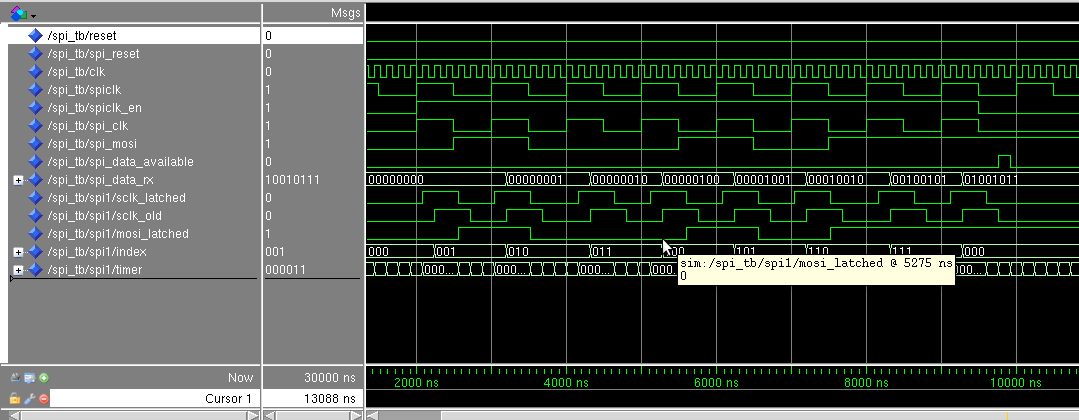
\includegraphics[width=\textwidth]{resource/waveSPI2.png}
	\caption{Een fragment van de wave van de SPI module.}
	\label{fig:waveSPI2}
\end{figure}

%Synthese AF
\subsection{Synthese en lay-out}
\label{sec:synthese en lay-out} 
Na uitvoering van de synthese op de SPI module blijkt dat de SPI een redelijk compacte module is. Door bij de synthese gebruik te maken van compile\_ultra verkregen we een totaal celloppervlak van 695 transistoren. Na met row placer handmatig de cellen te hebben geplaatst, hierbij is de optie "vary distance" uitgeschakeld, leverde de lay-out met trout een totaal van 2628 transistoren op. Van deze tranasistoren worden er een aantal van 1385 transistoren daadwerkelijk gebruikt. Dit levert een effici\"entie op van 52.70\%.   %verwerk hier de gegevens die je krijgt na synthese 

%Switchlevel test AF
\subsection{Switch-level simulatie}
De switch-level simulatie vergelijkt de simulatie op het transistor niveau met de simulatie op VHDL niveau. De resultaten van de gesynthetiseerde schakeling, die gesimuleerd is met SLS, wordt vergelken met de resultaten van de gesimuleerde testbench in ModelSim. Het verkregen switch-level resultaat, zie figuur \ref{fig:switchlevelSPI}, komt overeen met het al eerder verkregen ModelSim resultaat. Ook is er nog gebruik gemaakt van de optie compare. Deze gaf allemaal OK's terug (op de eerste na, maar dit hoort). Hieruit kunnen we concluderen dat de synthese van de SPI module goed is verlopen. 

\begin{figure}[H]
	\centering
	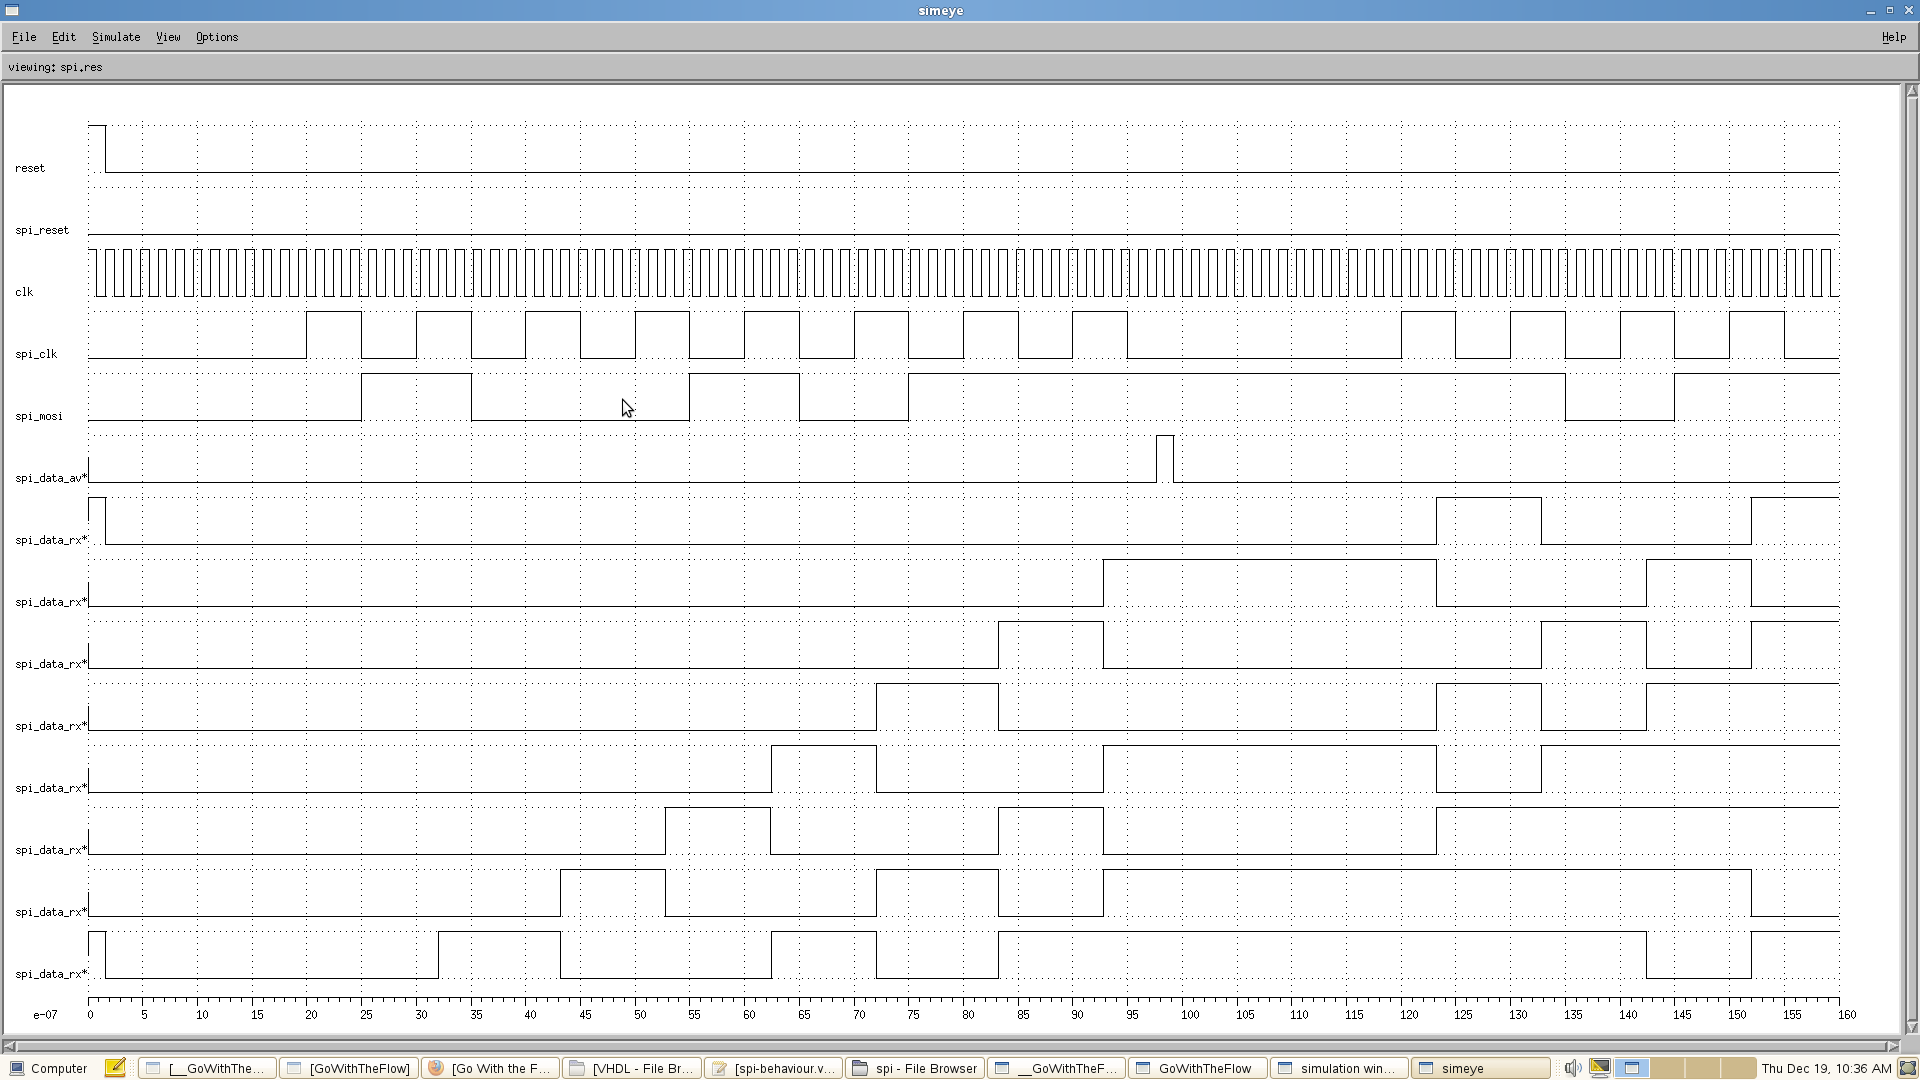
\includegraphics[width=\textwidth]{resource/switchlevelSPI.png}
	\caption{Het switch-level resultaat van de SPI module.}
	\label{fig:switchlevelSPI}
\end{figure}

%Conclusie AF
\subsection{Conclusie}
Alle gemaakte simulaties van de SPI module leverde uiteindelijk het gewenste resultaat op. Naar aanlieiding hiervan kan dan dus de cunclusie worden getrokken dan de SoG-implementatie van de module, op de gefabriceerde chip, zou moeten werken. Weliswaar is er ook wel een minpuntje binnen deze module. Dit is de effici\"entie van de module. Helaas, zoals al te lezen was in \ref{sec:synthese en lay-out}, blijft de effici\"entie met 52.70\% wat aan de lage kant. Hierdoor neemt de module helaas meer ruimte in beslag op de chip, dan dat nodig zou zijn als we een hogere effici\"entiegraad hadden gehaald. De transistoren die nu nodig zijn voor de SPI module, maar niet gebruikt worden, had misschien nog iets anders leuks mee gedaan kunnen worden. 


\end{document}
